% !TeX spellcheck = <none>
	
	%% bare_conf.tex
	%% V1.3
	%% 2007/01/11
	%% by Michael Shell
	%% See:
	%% http://www.michaelshell.org/
	%% for current contact information.
	%%
	%% This is a skeleton file demonstrating the use of IEEEtran.cls
	%% (requires IEEEtran.cls version 1.7 or later) with an IEEE conference paper.
	%%
	%% Support sites:
	%% http://www.michaelshell.org/tex/ieeetran/
	%% http://www.ctan.org/tex-archive/macros/latex/contrib/IEEEtran/
	%% and
	%% http://www.ieee.org/
	
	%%*************************************************************************
	%% Legal Notice:
	%% This code is offered as-is without any warranty either expressed or
	%% implied; without even the implied warranty of MERCHANTABILITY or
	%% FITNESS FOR A PARTICULAR PURPOSE! 
	%% User assumes all risk.
	%% In no event shall IEEE or any contributor to this code be liable for
	%% any damages or losses, including, but not limited to, incidental,
	%% consequential, or any other damages, resulting from the use or misuse
	%% of any information contained here.
	%%
	%% All comments are the opinions of their respective authors and are not
	%% necessarily endorsed by the IEEE.
	%%
	%% This work is distributed under the LaTeX Project Public License (LPPL)
	%% ( http://www.latex-project.org/ ) version 1.3, and may be freely used,
	%% distributed and modified. A copy of the LPPL, version 1.3, is included
	%% in the base LaTeX documentation of all distributions of LaTeX released
	%% 2003/12/01 or later.
	%% Retain all contribution notices and credits.
	%% ** Modified files should be clearly indicated as such, including  **
	%% ** renaming them and changing author support contact information. **
	%%
	%% File list of work: IEEEtran.cls, IEEEtran_HOWTO.pdf, bare_adv.tex,
	%%                    bare_conf.tex, bare_jrnl.tex, bare_jrnl_compsoc.tex
	%%*************************************************************************
	
	% *** Authors should verify (and, if needed, correct) their LaTeX system  ***
	% *** with the testflow diagnostic prior to trusting their LaTeX platform ***
	% *** with production work. IEEE's font choices can trigger bugs that do  ***
	% *** not appear when using other class files.                            ***
	% The testflow support page is at:
	% http://www.michaelshell.org/tex/testflow/
	
	
	
	% Note that the a4paper option is mainly intended so that authors in
	% countries using A4 can easily print to A4 and see how their papers will
	% look in print - the typesetting of the document will not typically be
	% affected with changes in paper size (but the bottom and side margins will).
	% Use the testflow package mentioned above to verify correct handling of
	% both paper sizes by the user's LaTeX system.
	%
	% Also note that the "draftcls" or "draftclsnofoot", not "draft", option
	% should be used if it is desired that the figures are to be displayed in
	% draft mode.
	%
	\documentclass[conference, letterpaper]{IEEEtran}
	\usepackage{booktabs}
	\usepackage[rflt]{floatflt}
	\usepackage{frame,caption,subcaption,calc}
	\usepackage{mathrsfs}
	\usepackage{array}
	\usepackage{amsmath,amssymb}
	\usepackage{color}
	\usepackage{setspace}
	\usepackage{stfloats}
% stfloats.sty was written by Sigitas Tolusis. This package gives LaTeX2e
% the ability to do double column floats at the bottom of the page as well
% as the top. (e.g., "\begin{figure*}[!b]" is not normally possible in
% LaTeX2e). It also provides a command:
%\fnbelowfloat
	\usepackage{fancyhdr}
%	\usepackage[caption=false,font=footnotesize]{subfig}
	\newcommand{\argmax}{\operatornamewithlimits{arg\,max}}
	% correct bad hyphenation here
	\hyphenation{op-tical net-works semi-conduc-tor}
	
	%\usepackage{subcaption}
	
	% *** GRAPHICS RELATED PACKAGES ***
	%
	\ifCLASSINFOpdf
	   \usepackage[pdftex]{graphicx}
	\else
	\fi
	
	
	%
	
	\renewcommand{\thispagestyle}[2]{} 
	
	
	\fancypagestyle{plain}{
	        \fancyhead{}
	        \fancyhead[C]{first page center header}
	        \fancyfoot{}
	        \fancyfoot[C]{first page center footer}
	}
	\pagestyle{fancy}
	
	
	\headheight 20pt
	\footskip 20pt
	
	\rhead{}
	
	%Enter the first page number of your paper below
	\setcounter{page}{1}
	
	%Header
	\fancyhead[R]{\textit{Intelligent Systems Conference 2018 \\ 6-7 September 2018 $|$ London, UK}}
	\renewcommand{\headrulewidth}{0pt}
	
	%Footer
	\fancyfoot[C]{IEEE}
	\renewcommand{\footrulewidth}{0.5pt}
	\fancyfoot[R]{\thepage \  $|$ P a g e }
	
	
	\begin{document}
	
	%
	% paper title
	% can use linebreaks \\ within to get better formatting as desired
	\title{Guess my power: A computational model to simulate a partner's behavior in the context of collaborative negotiation}
	
	
	% author names and affiliations
	% use a multiple column layout for up to three different
	% affiliations
	\author{\IEEEauthorblockN{Lydia OULDOUALI}
	\IEEEauthorblockA{LIMSI-CNRS, UPR 3251, Orsay, France\\
	Universit\'e Paris-Sud, Orsay, France \\
	Email: ouldouali@limsi.fr}
	\and
	\IEEEauthorblockN{Nicolas Sabouret}
	\IEEEauthorblockA{LIMSI-CNRS, UPR 3251, Orsay, France\\
	Universit\'e Paris-Sud, Orsay, France \\
	Email: nicolas.sabouret@limsi.fr}
	\and
	\IEEEauthorblockN{Charles Rich}
	\IEEEauthorblockA{	Worcester Polytechnic Institute\\ Worcester, Massachusetts, USA\\
	Email:rich@wpi.edu}}
	
	% conference papers do not typically use \thanks and this command
	% is locked out in conference mode. If really needed, such as for
	% the acknowledgment of grants, issue a \IEEEoverridecommandlockouts
	% after \documentclass
	
	% for over three affiliations, or if they all won't fit within the width
	% of the page, use this alternative format:
	% 
	%\author{\IEEEauthorblockN{Michael Shell\IEEEauthorrefmark{1},
	%Homer Simpson\IEEEauthorrefmark{2},
	%James Kirk\IEEEauthorrefmark{3}, 
	%Montgomery Scott\IEEEauthorrefmark{3} and
	%Eldon Tyrell\IEEEauthorrefmark{4}}
	%\IEEEauthorblockA{\IEEEauthorrefmark{1}School of Electrical and Computer Engineering\\
	%Georgia Institute of Technology,
	%Atlanta, Georgia 30332--0250\\ Email: see http://www.michaelshell.org/contact.html}
	%\IEEEauthorblockA{\IEEEauthorrefmark{2}Twentieth Century Fox, Springfield, USA\\
	%Email: homer@thesimpsons.com}
	%\IEEEauthorblockA{\IEEEauthorrefmark{3}Starfleet Academy, San Francisco, California 96678-2391\\
	%Telephone: (800) 555--1212, Fax: (888) 555--1212}
	%\IEEEauthorblockA{\IEEEauthorrefmark{4}Tyrell Inc., 123 Replicant Street, Los Angeles, California 90210--4321}}
	
	
	
	
	% use for special paper notices
	%\IEEEspecialpapernotice{(Invited Paper)}
	
	
	
	
	% make the title area
	\maketitle
	
	
	\begin{abstract}
		%\boldmath
	%	Interpersonal dominance relation has a major effect on the outcome of a negotiation. It has been shown that when participants adopt complementary dominance behaviors (one being dominant and the other being submissive), they reach mutually beneficial outcomes and this increases their reciprocal likings. 
	We present in this paper a computational model of collaborative negotiation capable of guessing the behavior of powed expressed by his partner.
	Our model is a straight continuation of our model of negotiation based on power \cite{ouali2017computational}. We present a model inspired from Theory of Mind  based on simulation that allows an agent to evaluate its interlocutor's level of power at each negotiation turn. We show on agent-agent simulation that the system correctly predicts the interlocutor's power. 
	\end{abstract}
	% IEEEtran.cls defaults to using nonbold math in the Abstract.
	% This preserves the distinction between vectors and scalars. However,
	% if the conference you are submitting to favors bold math in the abstract,
	% then you can use LaTeX's standard command \boldmath at the very start
	% of the abstract to achieve this. Many IEEE journals/conferences frown on
	% math in the abstract anyway.
	
	% no keywords
	
	
	\begin{IEEEkeywords}
		
		Human agent interaction ; Collaborative negotiation; Interpersonal relation of power;Reasoning about other; Theory of mind
	\end{IEEEkeywords}
	
	
	% For peer review papers, you can put extra information on the cover
	% page as needed:
	% \ifCLASSOPTIONpeerreview
	% \begin{center} \bfseries EDICS Category: 3-BBND \end{center}
	% \fi
	%
	% For peerreview papers, this IEEEtran command inserts a page break and
	% creates the second title. It will be ignored for other modes.
	\IEEEpeerreviewmaketitle
	\section{Introduction}
		Recent years have witnessed substantial growth in research on interactions between humans, intelligent agents and robots. Several new applications require agents and human user to collaborate in order to achieve shared goals and tasks. These include agents such as an \textit{eCoach} collaborating with a patient to choose a course of treatment from among many viable options \cite{robertson2015visual}, or an educational agent collaborating with a student to resolve problems \cite{howard2017shifting} along side with companions for the eldery \cite{sidner2014robotic}. 
		In such situations, users might have to negotiate with the conversational agent regarding the plan that achieves their common goals in such way that both satisfies them. This type of negotiation is called \emph{"Collaborative negotiation"}. It assumes that each participant is driven by the goal of finding a trade-off that satisfies best the interests of all the participants as a group, instead of one that maximizes his own interest \cite{sidner1994artificial,chu1995response}.
	
		However, negotiation is a multifaceted process which also involves social interaction and affects, as well as personal preferences and opinions  \cite{bro2010affective}. Several research considered the role of social behavior in the negotiation process. For instance, \cite{de2011effect} studied the impact of emotions of anger and happiness on the outcome of the negotiation.  \cite{kraus1995designing} developed an agent that behaves according to different personalities and has a learning mechanism to learn the personality of its opponents. 
	
		One key element in the social aspect of negotiation, is the interpersonal relation between the participants. Indeed, research in social psychology have demonstrated that the relation of dominance affects the perception of the negotiation process \cite{van2006power}.  
		Negotiating parties often differ in terms of dominance and this difference exerts an important influence on the behavior of participants. Negotiators build different negotiation's strategies depending on their relative dominance. This influences directly the outcomes of the negotiation. More precisely, Tidens \cite{tiedens2003power} showed that dominance complementarity (\emph{i.e.} one negotiator exhibits dominant behaviors while the other one responds with submissive ones) leads the negotiators to reach mutually beneficial outcomes and increases their reciprocal likings. \cite{wiltermuth2015benefits,tiedens2003power}.
	
		When building conversational agents that collaborate with a human user, it is important to take into account the interpersonal relationship established between the negotiators.
		 We focus in this paper on the relation of dominance. Burgoon \cite{burgoon1998nature} defines interpersonal dominance as expressive, relationally based communicative acts by which behaviors of power are exerted and influence achieved. They further define dominance as a dyadic variable in which control attempts by one individual are accepted by the partner, which means if one individual expresses behaviors of high power, the interactional partner will adapt with a low power behavior. 
	
		To express those behaviors of power, we designed a model of collaborative negotiation that allows an agent to express its power through negotiation strategies \cite{ouali2017computational}. We showed that human observers correctly perceived the power expressed by the agent.
		The next step is to extend this model in order to simulate an interpersonal relation of dominance between the agent and the user. This means that if one negotiator exerts behaviors of high power, its partner has to adapt in order to exert complementary behaviors of low power, and vice versa.
		
		\begin{figure*}[h]
			\centering
			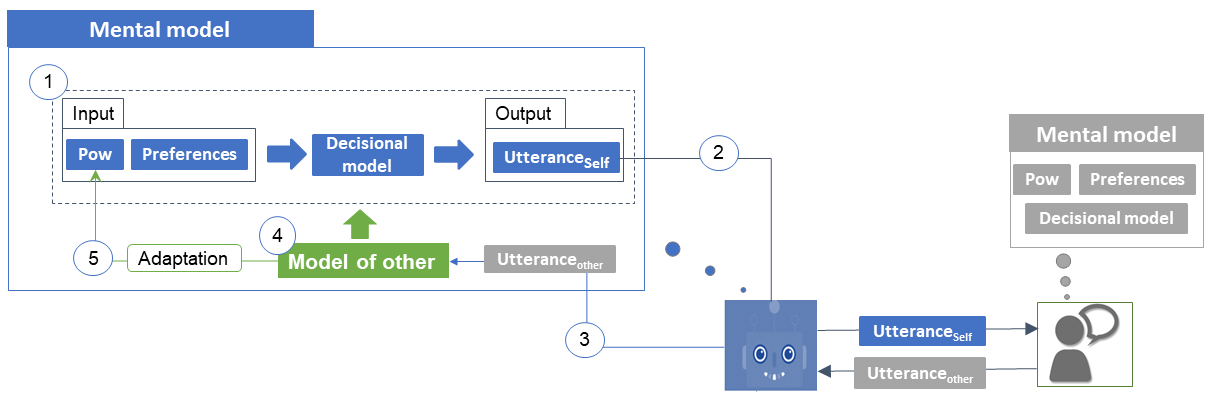
\includegraphics[width=0.8\linewidth]{figs/model/general.png}
			\caption{Model of collaborative negotiation with a model of other. Process of decision step by step} 
			\label{fig:schema-general}
		\end{figure*} 

	
		Our work aims at developing such an agent that is capable of evaluating and adapting his social behavior to the degree of power expressed by interlocutor. We propose a model of theory of mind based on \emph{simulation-theory (ST)} \cite{gordon1986folk} to evaluate the behavior of the partner. \emph{ST} suggests that humans, have the ability to project oneself in the other person’s shoes \cite{shanton2010simulation}. Therefore, we can simulate his or her mental activity with our own capacities for practical reasoning. It allows us to mimic the mental state of our interactional partner \cite{harbers2009modeling}.%\cite{http://ii.tudelft.nl/~maaike/papers/Iat_2009.pdf}
		  
		This paper describes our model of \emph{ST} that allows the agent to evaluate the behavior of its interlocutor and to reason about it in order to predict its intentional power as presented in the figure~\ref{fig:schema-general}. The agent assumes that its interlocutor has a similar decision's model based on power. Therefore, for each enunciated utterance by the user, the agent tries to guess the behavior of power that its partner intends to express. 
		 %In addition, we present the first step of our validation process, that aims to validate the accuracy of prediction made on the partner's behaviors. We study in the context of agent/agent interaction, in which one agent is implemented with our model of \emph{ST}, the degree of exactitude the agent guessed its interlocutor's behaviors of power. 

		The paper is organized as follows. Section II gives an overview of previous automated negotiation agents with theory of mind and other related work on social behavior recognition. In section III, we briefly present our model of dialogue for collaborative negotiation. We show that extending this model with a theory of mind raises computational issues. We propose a new model to evaluate the dominance of the interlocutor, based on reasoning with uncertainty. Section IV presents an evaluation of this new model in the context of agent-agent negotiation. We show that the system correctly predicts the interlocutor's power in spite of the restrictions on the model. In section V, we discuss the future use of this new model for building an adaptive negotiator agent.
	
	
	\section{Related works}
	
	%https://www.ncbi.nlm.nih.gov/pmc/articles/PMC3737477/ pour plus d'exemple de tom 
	In social interactions in general and negotiation in particular, reasoning about the beliefs, goals, and intentions of others is crucial. People use this so-called theory of mind \cite{premack1978does} or mentalizing to understand why others behave the way they do, as well as to predict the future behavior of others. Therefore, various negotiation models use theory of mind approaches to create  more realistic models of negotiation. 
	
	For instance, Pynadath \textit{et al} \cite{pynadath2013you} showed the advantages of theory of mind on negotiation even with an overly simplified model. They observed significant similarities between	the partner behaviors and the agent's idealized expectations. Moreover, deviations in expectations about the other did not affect the agent performances and played in some cases in the advantage of the agent.
	
	De Weerd \textit{et al} \cite{de2013higher} also investigated the use of high-order theory of mind in mixed-motive situations where cooperative and competitive behaviors play an important role. They found that the use of first-order and second-order theory of mind allow agents to balance competitive and cooperative	aspects of the game. This prevents agents from breaking down compared to  agents without theory of mind.
	
	
	Both approaches only focus on rational behaviors and exclude social aspects. However, the impact of social behaviors has been extensively debated in social psychology. Among such works, various researches have been investigating emotion recognition in negotiation; the effects of one individual's	emotions on the other's social decisions and behavior during the negotiation. Moreover, they investigate how theses resource of information are integrated.
	For example, Elfenbein\textit{ et al} \cite{elfenbein2007reading} proved that  emotion recognition accuracy is positively correlated to  better performances in negotiation.
	
	In the same vein, several researches suggested that anger expression has effects on the negotiation \cite{sinaceur2006get,van2010interpersonal,ferguson2004social}. For example, VanKleef \cite{van2004interpersonal} demonstrated that negotiators monitor their opponent's emotions and use them to estimate the opponent's limits, and modify their demands according to the presumed location of those limits. As a result, negotiators concede more to an angry opponent than to a happy one. 
	
	
	accordingly, reasoning about the social behaviors is important for the perspective of constructing negotiators agents. \cite{alfonso2015emotional} proposed a model that can observe and predict other's agents emotional behaviors: the three step method revises the agent's  beliefs by integrating a Bayesian model which infers probabilities about the emotional behaviors of other's agents and computes probabilistic prediction about their appraisals.
	
%	Marcella \textit{et al} \cite{klatt2011negotiations} proposed a model of negotiation in the context of aid prevention. The model tries to combine handling of emotions with general structures of negotiations. 
	
	In the context of our work, we focus on the impact of dominance in the negotiation. Dominance as an interpersonal relation is defined by burgoon \cite{burgoon1998nature} as expressive, relationally based communicative acts by which power is exerted and influence achieved. Furthermore, it is a dyadic variable in which control attempts by one individual are accepted by the
	interactional partner \cite{dunbar2005perceptions}. For this reason, we focus on dominance complementarity between a negotiator agent and a human user in the context of collaborative negotiation. 
	
	Dominance complementarity is characterized by one person in a dyadic interaction behaving dominantly and his counterpart behaving submissively \cite{tiedens2003power} and those behaviors have been investigated in the context of negotiation. \cite{tiedens2003power} showed that when complementarity occurs in an interaction, people feel more comfortable and helps to create interpersonal liking relation.
	Moreover, \cite{wiltermuth2015benefits} showed that dominance complementarity can positively improve coordination and by consequences improve objective benefits.
	
	Our goal is to create a model of negotiation in which the agent adapts its negotiation strategies to the relation of dominance established with the user. Therefore, the agent has to reason about user's behaviors of \emph{power} to understand the level of dominance or submissiveness expressed. The agent then adopt a complementary strategy in order to complement the user behaviors and establish the relation of dominance.
	
	We present in this paper a model of theory of mind that builds beliefs about the user behaviors of power in order to predict his behavior of dominance. We propose to use our model of negotiation based on power in order to reason about the user behaviors. 
	
	
	\section{Model of collaborative negotiation}
	The goal of our work is to simulate an interpersonal relation of dominance. We allow the agent to adapt its behaviors of power to complement its partner's behavior. We use a model inspired form simulation theory to guess the power of the partner. To this aim, we will use and adapt our model of collaborative negotiation to guess the partner's behavior. In this model of collaborative negotiation, the decisional process is governed by the power the agent seeks to express. Indeed, the strategies expressed by the agent are influenced by power. These strategies were designed based on researches from social psychology which studied the impact of power on negotiator's strategies. 
	%Indeed, in addition the agent's preferences,the decisional process of this model takes into account the power of this agent to make decisions during the negotiation.
	
	In this section, we present an overview of our collaborative negotiation model. Indeed, it is not necessary to have a complete knowledge of this dialogue model to understand the simulation presented here. However, some elements are required to explain our approach. This section briefly presents the main principles of the collaborative negotiation dialogue model. The detailed presentation is explained in a previous work \cite{ouali2017computational}.
	

	
	\subsection{Dialogue model}
	
	\label{sec:dialogue-model}
	
	The goal of a negotiation is to choose an option in a set of possible options $\mathcal{O}$. Each option $o\in\mathcal{O}$ is defined as a set of values $\{v_1, ..., v_n\}$ associated to criteria $\{C_1, ..., C_n\}$ that reflect the option's characteristics.  
	For instance, in a negotiation about restaurants, the criteria might be the type of cuisine and the price, we could have the option: $(French,Expensive)$.
	
	The agent is provided with a set of partial or total ordered preferences $\prec_i$ defined for each criterion $C_i$. Using these preferences, the agent can compute a score of satisfaction $sat(v)$ for each value of each criterion. The satisfaction of a value $v \in C_i$ is computed as the number of values that the agent prefers less in the preferences order $\prec_i$. The notion of satisfaction represents the score of liking for the value. The closer the satisfaction of a value $v$ gets to 1, the more the agent likes $v$.
	 
	 
	For example, let's consider the criteria of $cuisine$ defined with the following values: $\{$\emph{french$(fr)$, italian$(it)$, japanese$(jap)$, chinese$(ch)$}$\}$. In addition, the agent has a total order of preferences on these values $\prec_{cuisine}$$=\{ch$$\prec$$jap, jap$$\prec$$it, it$$\prec$ $fr\}$. Based on this order of preferences $\prec_{cuisine}$, the agent is able to compute the value of satisfiability associated to each value as presented in table \ref{tab:sat}.
	
	\begin{table} [h]
		\centering
				\large
		\begin{tabular}{ |c|c|c|c|c| }
		\hline
		value & $ch$ & $jap$ & $it$ & $fr$ \\	
		\hline
		sat(value) & 0 & 0.33 & 0.66 & 1 \\
		\hline
	\end{tabular}
		\caption{$Sat$ computed on the set of preferences $\prec_{cuisine}$.}
		\label{tab:sat}

	\end{table}


	
	The domain of negotiation includes a \emph{communication model}. This model enables the agent to communicate with its partner throughout text based \textit{utterances}. 
	Each one is associated with a natural language formulation.% The details are presented in \cite{ouali2017computational}.
	
	To keep the model as generic as possible, we defined five utterances types grouped in three different categories: 
	\begin{itemize}
			\item \textbf{Information moves} (\textit{AskValue/AskCriterion} and \textit{StateValue}) are used to exchange information about the participant's likings. They are used to express what the agent likes or do not like (\emph{e.g} \textit{I (don't)like Chinese restaurants}).
			
			\item 	\textbf{Negotiation moves} (\textit{Propose}, \textit{Accept} and \textit{Reject}) allow the agent to make or to answer to proposals. The agent can propose, accept and reject, both values (``Let's go to a Chinese restaurant'') or options (``Let's go to \emph{Chez Francis}'').	
			
			\item 	\textbf{Closure moves} (\textit{NegotiationSuccess} or \textit{NegotiationFailure}) are used to end the dialogue.
	\end{itemize}

	
	\subsection{Decision based on power}
	\label{sec:dec}
	The decision making process is designed to consider, in addition to preferences, the power of the agent as presented in the \textit{step 1} of the figure \ref{fig:schema-general}. 
	Therefore, the agent is initiated with a value of power $pow \in [0,1]$. 
	
	We present in this section, the decisional model, which relies on three elements. We will explain how the principles of power inspired from social psychology literature influence this decisional process.

	
	\subsubsection{Satisfiability}
	\label{sec:sat}
	The value of satisfiability is associated to the \emph{StatePreference(v)} utterance that allows the agent to express his likings. As shown by \cite{de1995impact}, high-power negotiators are more demanding than low-power ones.
	We capture this principle by implementing a set of the agent's satisfiable values, named $S$, that varies depending on the level of power $pow$. It is computed as follows:

	\begin{equation}
		\forall v,\hspace{2mm} v\in S\hspace{2mm}\mathrm{iff}\hspace{2mm}sat(v) \geq pow
	\end{equation}
	
	For example, let us consider the preference set $\prec_{cuisine}$ whose values of satisfiability are given on table~\ref{tab:sat}. Assume a first agent Bob with a value of power $pow = 0.7$. We can compute, using the above function, that bob likes only $french$ cuisine $S= \{fr\}$. On the contrary, a second agent Arthur with a smaller value of power $pow=0.4$ will have its set of satisfiable values initiated to $S= \{fr, it\}$. 
	
    This set $S$ is used directly to compute the likability of values expressed in the \emph{StatePreference} utterances.
	
	\subsubsection{Acceptability}
	\label{sec:acc}
	In collaborative negotiation, both negotiators might have to reduce their level of demand over time because they want to reach a mutual agreement. The level of concessions expressed in a negotiation is affected by power. It was demonstrated that low-power negotiators tend to make larger concessions than high-power negotiators \cite{de1995impact}.
	
	We designed a function that decreases the agent level's of demand during the negotiation, specifically, when the negotiation is not converging.  To model this behavior, we use a \emph{concession curve}, named $self(t)$ . %and illustrated in Figure \ref{fig:conc}.
	We define this function to be a time varying function of $pow$ which decreases over time $t$ and follows the concession curve. In the beginning, $self(0) = pow$ and when the negotiation evolves without converging, the function decreases as illustrated in the figure \ref{fig:conc}.
	
	
	\begin{floatingfigure}[l]{1.2in}
		\captionsetup{justification=centering}
		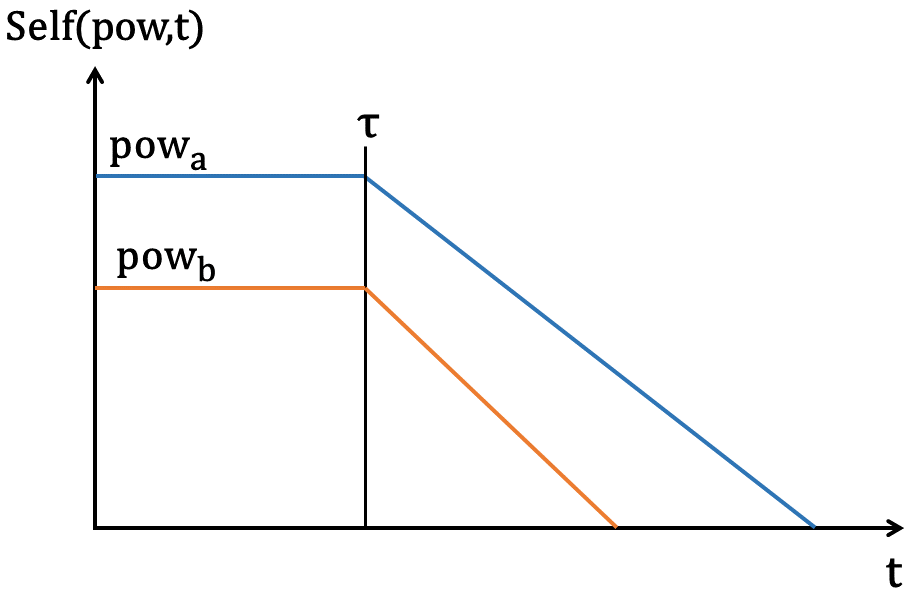
\includegraphics[width=1.2in]{figs/s3.png}
		\caption{\label{fig:conc}Concession curve}
	\end{floatingfigure} 
	
	
%	This function is designed to evaluate the acceptability of a proposal. Indeed, during the process of negotiation, the agent makes decisions about the proposals it receives by its partner. It might express an \emph{Accept} or \emph{Reject}. In the case where the negotiation is not converging, the agent has to lower his level of demand and makes concessions. Therefore, t
	The agent uses the value of $self$ to directly answer a \emph{Propose(v)} utterance. We say that the value $v$ is \emph{acceptable} at time $t$, and we note $v \in Ac(t)$, when:
	\begin{equation}
	v\in Ac(t)\hspace{2mm}\mathrm{iff}\hspace{2mm}sat(v) \geq self(t)
	\end{equation}
	
	The agent will answer with an \emph{Accept} to a proposal only if the value is acceptable, and will answer with a \emph{Reject} otherwise. Also note that, when building proposals (i.e. \emph{Propose} utterances) the agent can only propose a value that is acceptable.
	
	Finally, it is important to note that the set $Ac(t)$ grows over time: as the negotiation evolves, the agent might accept proposals which are not satisfiable, as a consequence of making concessions. We denote $M(t)\subsetneq Ac(t)$ the set of not-satisfiable values that can became acceptable due to concessions: $M(t)=Ac(t)\setminus S$.

	For example, in the context of negotiation with a set of preferences $\prec_{cuisine}$ and $pow= 0.6$, as illustrated in Table~\ref{tab:sat}. The set of satisfiable and acceptable values are initiated to $S=Ac(t)=\{it,fr\}$ and $M= \emptyset$. 
	However, due to concessions, the value of self, initially to $self(0)=0.6$, reduces to $self(t)=0.3$. Thus, values which are not satisfiable are now acceptable. Therefore, the set $Ac(t)$  is updated  $Ac(t)=\{it,fr,jap\}$ and by consequences $M=\{jap\}$. 
	
	\subsubsection{Lead of the dialogue}
	De Dreu \textit{et al} showed that the participant with higher power tends to lead the dialogue and to focus on the negotiation convergence \cite{magee2007power,de2004influence}. On the opposite, low power negotiators focus on building an accurate model of their partner's preferences in order to make the fairest decision \cite{de1995impact}. This leads them to ask more questions about other preferences
	
	In our model, this means that agents with high values of power ($pow>0.5$) will select \emph{Propose} moves more often. Indeed, to make the negotiation converge, the agent has to keep making proposals until a compromise that satisfies the agent and its partner is found.
	On the contrary, agents with low power will select \emph{AskPreferences} utterances more often to collect information. A detailed presentation of the utterance selection is presented in \cite{ouali2017computational}.
		
	
	\subsubsection{Example of dialogue}	
		We present an example of dialogue generated with two agents implement with our model of dialogue. Agent$A$ adopts a dominant behavior $pow_A =0.7$ and the agent$B$ follows a submissive behavior $pow_B =0.4$. The dialogue is illustrated on Figure \ref{fig:ex-dia}.
		
		\begin{figure}
		\fbox{ \begin{minipage}{.48\textwidth}
				\slshape
				\setstretch{1.65}
							%\begin{addmargin}[1em]{2em}% 1em left, 2em right
								\textbf{A:} "Let's go to a restaurant on the south side."
								
								\hspace*{3mm}\textbf{B:} "I don't like restaurants on the south side, let's choose something else."
							
								
								\textbf{A:} "Let's go to a modern restaurant."
								
								
								\hspace*{3mm}\textbf{B:} "Okay, let's go to a modern restaurant."
								
								\textbf{A: }"Let's go to a French restaurant."
								
								\hspace*{3mm}\textbf{B:} "Okay, let's go to a French restaurant."
								
								\textbf{A:} "Let's go to the Maison blanche restaurant. It's a modern, cheap French restaurant on the south side."
								
								\hspace*{3mm}\textbf{B:} "What kind of cost do you like?"
								
								\textbf{A:} "I like cheap restaurants."
								
								\hspace*{3mm}\textbf{B:} "Do you like expensive restaurants?"
								
							\textbf{A:} "Let's go to the Maison blanche restaurant. It's a modern, cheap French restaurant on the south side."
								
								\hspace*{3mm}\textbf{B:} "Okay, let's go to the Maison blanche restaurant."
						%	\end{addmargin}
					\end{minipage}
				}
			
		\caption{\label{fig:ex-dia}Example of dialogue between agents \emph{A} and \emph{B} implemented with our model of collaborative negotiation.}
	\end{figure}


	\section{Beliefs about other: general algorithm}
	
	In order to figure out the value of power expressed by the user, the agent has to understand the decisional model of the user. To this goal, we propose to use a Theory of Mind (ToM) approach \cite{premack1978does} based on simulation (\emph{ST}) to establish and maintain representations of the mental states of its human counterpart as illustrated in the \emph{step-4} in the figure\ref{fig:schema-general}. 
	The mental state requires to model the inputs necessary to reason during the negotiation. The idea is to consider different hypotheses about the user's mental state, including his/her value of power and its preferences. Using the agent's decision model, we simulate the possible utterances produced by each hypothesis. 
	We then compare the results of this simulation with the actual utterance expressed by the user ($Utterance_{other}$) in \textit{step 3}. This gives information about the possible values of power. The principle is illustrated on Figure~\ref{fig:tom}.
	
	\begin{figure*}
		\centering
		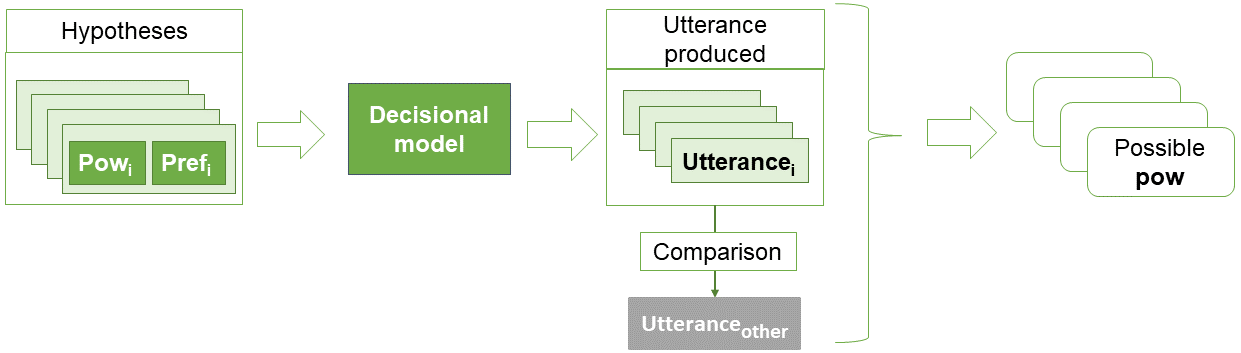
\includegraphics[width=0.8\linewidth]{figs/model/tom_select.png}
		\caption{Model of theory of mind to evaluate hypotheses on the power of the intertlocutor from its utterance} 
		\label{fig:tom}
	\end{figure*} 
	
	This approach, however, relies on a couple of strong assumptions. First, it assumes that the decision model is an accurate representation of the decisional process of the user. There is no way to guarantee this assumption. However, in our previous research \cite{ouali2017computational}, we showed that the behaviors of power expressed by agents are correctly perceived by human users. 
	%This is no proof that the model is similar to a human decision process, but the behaviors that it produces are at least coherent with the notion of dominance as human people understand it.
	
	The second assumption is that the system can build a model of the possible mental states of the interlocutor. Concretely, this means a value of $pow$ and a set of preferences $\prec_i$ for all criteria. 
	
	Based on these assumptions, we present the general algorithm of the user's model of mental state as follows:
	\begin{enumerate}
		\item Build a set $H_{pow}$ of hypothesis about power: $h\in H_{pow}$ represents the hypothesis $pow=h$. In our work, we consider only 9 values: 
		
		$H_{pow}=\{0.1, 0.2, \ldots, 0.9\}$.
		\item For each hypothesis $h$, build the set of all possible preferences $Prec_h$: the elements $p\in Prec_h$ are partial orders on the criteria.
		\item After each user utterance $u$, remove all elements in $Prec_h$ that are not compatible with $u$. Concretely, if the applicability condition of $u$ is not satisfied in $p\in Prec_h$, then $p$ must be removed from the candidate mental states.
		\item For each $h$, generate the corresponding utterance using $h$ as input for the decisional model.
		\item Compute a score $score(h)$ based on the size of remaining hypothesis $|Prec_h|$ that generate an output similar to the utterance, $Utterance_{other}$, enunciated by the user. 
		\item 	The hypothesis with the highest score is the most probable value for the user's power value.

		\begin{equation}
		pow_{other} = \operatorname*{arg\,max}_{h} (score(h))
		\end{equation}
		
	\end{enumerate}
		
	
	\subsection*{Simulation of the other's preferences}
	
		The representation of the user's preferences is a crucial input for the decisional model. In order to generate the set of possible preferences for each hypothesis, we need to consider all possible partial orders $\prec_i$ for each criterion $C_i$. 
		We can compute the size of the set of binary preferences based on the number of values, which is $(|C_i| + 1)!$ possible partial orders for each criteria. As a consequence, for a topic with $n$ criteria, there are $\prod_{i=1}^n (|C_i|+1)!$ different possible preference sets.
	
		If we consider a reasonable example, with 5 criteria. For each criteria, we consider approximatively 4 to 10 possible values each. The set of possible preferences that the agent has represent for the user's model, are between $24.10^9$ and $10^{38}$ possible preference sets. 
		We can easily conclude that it is not reasonable to consider all theses hypotheses, one by one, at each step of the dialogue.
	

		We conducted an analysis of our decisional model to define the need of preferences. As presented in section \ref{sec:dec}, the preferences are used to compute the \emph{satisfiability} of each value. %The value of \emph{satisfiability}
		 This value is necessary during the decisional process because it is required to build the set of satisfiable values $S$, and the set of acceptable values $Ac(t)$.   
		 
		 	\begin{table} [h]
		 		\centering
		 		\large
		 		\caption{$Sat$ computed on the set of preferences for two total ordered preferences sets.}
		 		\begin{tabular}{ |c|c|c|c|c| }
		 			\hline
		 			value & $ch$ & $jap$ & $it$ & $fr$ \\	
		 			\hline
		 			sat(value) $\prec_{cuisine}$ & 0 & 0.33 & 0.66 & 1 \\
		 			\hline
		 			sat(value) $\prec'_{cuisine}$ & 1 & 0.33 & 0 & 0.66 \\
		 			\hline
		 		\end{tabular}

		 		\label{tab:ex2_sat}
		 		
		 	\end{table}
	
		However, in the case of \underline{\textit{total ordered preferences}}, all the values are comparable, which means that they can be sorted by order of preferences, by calculating the number of predecessors, as in the example \ref{tab:sat}. Independently from the values themselves, by knowing the number of values, we can compute the value of \emph{satisfiability} of each value only from its rank of this in the order of preferences. For example, if we define a different set of preferences  on the criterion $cuisine$ $\prec'_{cuisine} = \{it$$\prec$ $jap, jap$$\prec$$ fr, fr$$\prec$$ch\}$, we will obtain similar values of satisfiability as presented in Table~\ref{tab:ex2_sat}. Indeed, the score of satisfiability for each value can be directly computed from the number of predecessor in the ranking. Therefore, in a total ordered preferences, we will always obtain the same values of satisfiability as presented in the table \ref{tab:poss}. 


	\begin{table}[h]
		\caption{Satisfiability depending on the rank for a 4-values criterion.}
		\label{tab:poss}
		\centering
		\large
		\begin{tabular}{ |c|c|c|c|c| }
			\hline				
			rank(value) & 1 & 2 & 3 & 4 \\
			\hline
			Nb predecessors & 3 & 2 & 1& 0 \\
			\hline
			$sat(value)$ & 0 & 0.33 & 0.66 &1 \\
			\hline
		\end{tabular}
	\end{table}
	
	As a consequence, for a given value of power $pow$, we can compute the number of satisfiable values $S$ without knowing the binary relations of preferences. For example, for the criterion $cuisine$ which have 4 values, for any given total ordered preference, and a value of $pow = 0.6$, we can deduct that the number of satisfiable values is always $|S| = 2$.
	
	Instead of calculating all the possible relations of preferences $\prec$, we can reduce the calculation to the set of possible satisfiable values.  Concretely, consider a criterion with $n$ number of values and total ordered preferences. For a given value of power $pow$, we obtain, $s$  the size of $S$. We have to generate only $\binom{n}{s}$ possibilities for the values of $S$ to consider. For example, for the criterion $cuisine$ and $pow =0.6$, we can generate all the possible satisfiable values as illustrated in table \ref{tab:sat_poss}.
		\begin{table}[h]
			\centering
			\caption{The possible sets $S$ for $cuisine$, with $pow=0.6$}
			\label{tab:sat_poss}
			\large
			\begin{tabular}{|c|c|c|}%|p{1.9cm}|p{2.25cm}|p{2cm}|p{2.25cm}|p{2cm}|p{2.25cm}| }
				\hline
				$S_1=(it,fr)$& $S_2=(it,jap)$ & $S_3=(it,ch)$\\
				\hline
				$S_4=(fr,jap)$ & $S_5=(fr,ch)$ & $S_6=(jap,ch)$ \\
				\hline
			\end{tabular}
		\end{table}
	
	This partial representation of preferences allows our model of the other to work with a reduced set of hypotheses, compared to the initial model with a complete representation of the preferences. If we consider the same example, with 5 criteria and 10 values per criterion, the maximum number of hypotheses to consider for a given value of power is $\binom{10}{5}=252$ (this value is maximum for $pow=0.5$).
 	However, simulating the behavior of the interlocutor with incomplete knowledge has two consequences. First, it requires to adapt the simulation model of the decision making to deal with the non-ordered sets of satisfiable and acceptable values. Second, it might affect the precision of the prediction of the interlocutor's power.

	In order to generate hypotheses about satisfiable values, given any criterion, we make the strong assumption that the interlocutor's preferences are \emph{total ordered}. Therefore, given a fixed value of $h \in H_{pow}$, we compute the number of satisfiable values named $s$ which is the size of all our hypotheses $S$ for this value of power. 
	We then built all possible combinations of satisfiable values noted $M_h()$ (see Table~\ref{tab:hypo}). This process is generalized to all the hypotheses of $H_{pow}$. We present in Table~\ref{tab:sat} an example of the generation of all the hypotheses possible for a criterion $cuisine$.
	
	\begin{table}[h]
		\centering
		\caption{Hypotheses on preferences for a 4-value criterion $cuisine$}
		\begin{tabular}{ |p{1.4cm}|p{1cm}|p{5cm}| }
			\hline
			& \multicolumn{2}{c|}{Hypotheses}  \\
			\hline
			Hypothesis & $h_i(pow)$ & Hypotheses on satisfiable values $ M_h(h_i)$\\
			\hline
			H1&0.3&$\{(fr,it,jap)\} , \{(fr,it,ch)\}$, $\{(fr,jap,ch)\}$,$\{(it,jap,ch)\}$ \\
			\hline
			H2&0.4&$\{(fr,it)\}, \{(fr,jap)\}, \{(fr,ch)\}$, $\{(it,jap)\},$ $\{(it,ch)\}$,$\{(jap,ch)\}$ \\
			\hline
			H3&0.5&$\{(fr,it)\}, \{(fr,jap)\}$,$\{(fr,ch)\}$, $\{(it,jap)\}$,$\{(it,ch)\}$,$\{(jap,ch)\}$\\
			\hline
			H4&0.6&$\{(fr,it)\}, \{(fr,jap)\}$, $\{(fr,ch)\}$, $\{(it,jap)\}$,$\{(it,ch)\}$,$\{(jap,ch)\}$ \\
			\hline
			H5&0.7&$\{(fr)\}, \{(it)\}, \{(jap)\}, \{(ch)\}$\\
			\hline
			H6&0.8&$\{(fr)\}, \{(it)\}, \{(jap)\}, \{(ch)\}$ \\
			\hline
			
			H7&0.9&$\{(fr)\}, \{(it)\}, \{(jap)\}, \{(ch)\}$ \\
			\hline
		\end{tabular}		
		\label{tab:hypo}
	\end{table}
	
	Using the model of hypotheses composed of hypotheses on power $h_{pow}$ and hypotheses on satisfiable values $ M_h(h_i)$ associated to each $h_i \in h_{pow}$, the agent has to simulate the behavior of its interlocutor at each turn of dialogue.  
	We present in the next section the adaptation of the decisional model to simulate the interlocutor behavior with partial knowledge.
	
	\section{Simulation of other with partial representation of preferences}
	\label{sec:simulation}
		After each dialogue turn in which an interlocutor expresses an utterance $utterance_{other}$, the agent uses its \emph{model of other} to update his hypotheses on the behavior related to power of its interlocutor $other_{pow}$. 
		Therefore, depending on the utterance's type, the agent computes, for each hypothesis, a score $score(h_i,t)$ which represents the accuracy of this hypothesis to the behavior expressed by the user. Then, the agent associates the value of power to the hypothesis that gets the best score at this turn:
			
			\begin{equation}
			pow_{other} = \operatorname*{arg\,max}_{h_i \in H_{pow}} (score(h_i,t))
			\end{equation}
		
	In this section, we present the process of simulation in which the agent predicts the behavior of power based on the received utterance. 
		
		\subsection{Lead of the dialogue}		
		As presented before, the choice of a specific utterance's type translates behaviors of power. Indeed, a high frequency of choosing \emph{proposal utterance} shows a behaviors of high-power. On the contrary, a high frequency of \emph{share preferences utterances} reflects behaviors of low-power.
		We note $history$ the list of utterances enunciated by the user. the value of power is computed from the ratio of \textit{propose} enunciated versus \textit{ask}.
		\begin{equation}
		pow_{other} = \left\{\begin{array}{ll}
		> 0.5 & \mathrm{if } \frac{history(Propose)}{hisotry} > 0.5\\
		\leq 0.5 & \mathrm{if  } \frac{history(Ask)}{hisotry} > 0.5
		\end{array}\right.
		\end{equation}
		
		Once, the list of possible hypotheses to consider is restricted, we update the hypotheses by taking into consideration the value associated to the expressed utterance.
		For example, suppose that the agent assumes that $\frac{history(Propose)}{hisotry} > 0.5$. Therefore, the agent will only considers the hypotheses $\{h_4 - h_9\}$ to compute the power of its interlocutor.
		
	\subsection{Share a preference}
		We consider that the interlocutor shares a preferences in two cases.
		First, when the interlocutor expresses a \emph{StatePreference(v,s)}, he shares a preference in a way where $v \in S$ (I like $v$) otherwise $v \notin S$ (I don't like $v$). 
		
		Second, based on our design, we consider that the interlocutor shares a preference when he/she rejects a proposal \emph{Reject(p)}. If a value is not acceptable, it is necessarily not satisfiable because $S \subset Ac(t)$. Thus, if $p\not\in Ac(t)$, then $p\not\in S$. 
		
		To compute whether a value $v \in C_i$ is satisfiable, we check for each hypothesis of power $h_i$, the set satisfiable values $S_i \in M_h(pow)$.
		Thus: 
			\begin{equation}
			sat_{S_i}(v)= \left\{\begin{array}{ll}
			True	 & \mathrm{if\ }  v \in S_i\\
			False & \mathrm{otherwise}
			\end{array}\right.
			\end{equation}
			
		Therefore, when the agent learns a new preference about its interlocutor, he updates his hypotheses as follows: 
		for each  $h_i \in H_{pow}$, we propose to update the agent's hypotheses $M_h(h_i)$ by removing all the hypotheses on preferences that are no longer consistent with the information acquired. 
		Then, we compute the score of each $h_i$ at the moment $t$ :
		
		$$score(h_i,t) = \frac{|M_h(h_i, t)|}{|M_h(h_i, init)|}$$
		
		\subsubsection*{\bf Example}
		
		Suppose that the interlocutor expresses $\emph{StatePreference(fr, true)}$, this means that the agent has to remove all the hypotheses where $fr \not\in S_i$. The update of each hypothesis and their respective scores are presented in Table~\ref{tab:update_hyp}. 
		
		For example, for $h_4$, out of the six initial hypotheses, the agent removes three: $(\{(it,jap)\}$, $\{(it,ch)\}$, $\{(jap,ch))$. In the end, $score(h_4) = 0.5$. 
	
		\begin{table}[h]
			\centering
			\caption{Hypotheses on preferences for a 4-value criterion $cuisine$}
			\begin{tabular}{ |p{1.4cm}|p{1cm}|p{3.2cm}|p{1.8cm}|}
				\hline
				& \multicolumn{3}{c|}{Hypotheses}  \\
				\hline
				Hypothesis & $h_i(pow)$ & Hypotheses on satisfiable values $ M_h(h_i)$ & $Score(h_i,t)$\\
				\hline
				H1&0.3&$\{(fr,it,jap)\}$, $\{(fr,it,ch)\}$, $\{(fr,jap,ch)\}$ & $3/4$ \\
				\hline
				H2&0.4&$\{(fr,it)\}$,$\{(fr,jap)\}$, $\{(fr,ch)\}$ & $0.5$ \\
				\hline
				H3&0.5&$\{(fr,it)\}$,$\{(fr,jap)\}$, $\{(fr,ch)\}$ & $0.5$\\
				\hline
				H4&0.6&$\{(fr,it)\}$,$\{(fr,jap)\}$, $\{(fr,ch)\}$& $0.5$ \\
				\hline
				H5&0.7&$\{(fr)\}$ & $1/4$\\
				\hline
				H6&0.8&$\{(fr)\}$ &$1/4$\\
				\hline
				
				H7&0.9&$\{(fr)\}$ &$1/4$\\
				\hline
			\end{tabular}		
			\label{tab:update_hyp}
		\end{table}
	
	\subsection{Proposals}
		When the interlocutor accepts (\emph{Accept(p)}) or proposes a proposal (\emph{Propose(p)}), means that the value is acceptable $p \in Ac(t)$. 
		The agent has to calculate for each $h_i \in H_{pow}$ the score of acceptability attributed to this value. 
		
		The set of acceptable values $Ac(t)$ depends on the value of $self(t)$, knowing that $self(t)$ decreases over time when the negotiation is not converging. Our goal is to capture the behaviors of concessions over time. Concretely, this means that the set of acceptable values $Ac(t)$ grows during the negotiation, and new values become acceptable noted $M(t)$. 
		
		Thus, for each hypothesis on power $h_i$, we associate a value $self_i(t)$ that represents the level of concessions at the current time. Using this value, and the set of satisfiable values (see Table~\ref{tab:poss}), the agent can compute the number of acceptable values $|Ac(t)_i|$, as presented in \ref{sec:acc}, and the number of the values which became acceptable due to concessions $|M(t)_i|$.
		
		Therefore, we propose to adapt the calculation of $acceptabilty$ only with partial knowledge available. For a hypothesis of power $h_i$, for each hypothesis on preferences $S_i \in M_h(h_i)$, and the list of accepted values during the negotiation $A$, the score that a value $p \in C_i$ is acceptable, is computed as follows:
		
		\begin{equation}
		Acc(p, h_i) = C_{|C_i|-(|S_i| + k)}^{|M_i(t)| - k}
		\end{equation}
		$k = |K| $ is the number of elements in the set $K=A \cap \overline S_i$, the set of accepted values which are not satisfiable. The score of acceptability is the number of possible sets $M_i(t)$ that are compatible with the value $p\in C_i$ (i.e. the value that was proposed or accepted by the interlocutor) and the hypothesis $S_i$.
		%Using this function, the agent can compute the $acceptability$ of each value of $cuisine$ for the the set $S_i$ relied to $h_4$. 
		

		In addition, we normalize this score of acceptability in order to have a coherent comparison between the different hypotheses (the number of hypotheses for each value of $pow$ can differ). Thus, given a hypothesis on power $h_i$, he score of acceptability is normalized by taking into account the ideal score of acceptability. We can compute the "best" score of acceptability a priori:
		
		$$I_{pow} = C_{|C_i|-|S_i|}^{|M_i(t)|}$$
		
		
		The final value of acceptability normalized is then:
		\begin{equation}
		score(h_i, t)= \left( \begin{array}{c}  \frac{1}{I_{pow}} \cdot \sum_{S_i \in M_h(h_i) } acc(p, h_i) 
		\end{array}\right) \frac{1}{| M_h(h_i)|}
		\end{equation}
		
			%	------------------------------------------------------------------------------------------------------------------------------
		
		\subsubsection*{\bf Example}
		
		The agent receives an \emph{Accept(jap)}. We take as example, $h_4$ to compute the values of acceptability of the value $jap$.

		With the partial representation of preferences, the agent only knows hypotheses about the sets $S_i \in M_h(h_i)$.
		In the case where there are no concessions ($self_i(t)=h_i$), the agent can compute the set of acceptable values because $|Ac_i(t)| = s$.
	
		However, if self decrease to $self_i(t)=0.3$, the number of acceptable values $|Ac_4(t)| = 3$. By consequence, the agent knows that a new value is acceptable which is also not satisfiable $|M_4(t)|=1$. 
		Moreover, the agent is not able to compute which value is now acceptable. For example, consider the first hypothesis on satisfiable values related to $h_4$; $S_i = \{fr, it\}$, the agent cannot compute which of the values $jap$ or $ch$ is now acceptable. Therefore, we compute the value of acceptability presented above that handle this uncertainty. 
		$ acc(jap, h4) = C^1_2 = 2$. The best score $I_{0.6}=2$. Thus, $score(h_4,t)= 1/6$
	

	
	% -----------
	\section{Evaluation}
	Section \ref{sec:simulation} presented a model based on \emph{ST} that aims to guess the behaviors of power expressed by an interlocutor. In order to assess the validity of our model with partial representation of preferences, we propose to simulate dialogues with two artificial agents. We can then compare the result of the prediction with the actual mental model of the interlocutor. We do not only evaluate the accuracy of our model of theory of mind, but also how fast it can predict the power of the interlocutor as well as the timeliness of the algorithm.
	
	\subsection{Method}
	We implemented two agents that have to negotiate over the topic of restaurants. In addition, each agent has to predict the behavior of power expressed by the other agent. 
	The first agent ($agent_A$) plays the role of a dominant agent, whereas, the second agent ($agent_B$) plays the role of a submissive agent.
	
	We manipulated two simulation parameters for the initialization of our agents.
	
	First, we variate the values of power assigned to each agent (named \emph{$pow_a$} and \emph{$pow_b$}), in order to study the accuracy of prediction in the different ranges of the spectrum of power as presented in Table~\ref{tab:powsettings}. For each behavior, we generated dialogues for each combination of values of power. 
	\begin{table}[h]
		\centering
		\caption{Initial condition's setting for the values of power} 
		\begin{tabular}{|l|cccc|}
			\hline 
			\textbf{Dominance value } &	\multicolumn{4}{c|}{ Initial values of power } \\
			\hline
			Dominant agent $pow_A$ & 0.3 & 0.4 & 0.5 &  \\
			\hline
			Submissive agent $pow_B$ & 0.6 & 0.7 & 0.8 & 0.9\\
			\hline
		\end{tabular}
		
		\label{tab:powsettings}
	\end{table}
	
	Second, we variate the initial preferences affected to each agent. More specifically, we generated different set of preferences that differs in their complexity. This means, that for each type of model of preferences, we variate respectively, the number of criteria discussed, and the number of values assigned to each criterion as presented in Table~\ref{tab:initP}. When the topic discussed has an important size of values to discuss, this implies that the agent has an important  number of hypotheses to consider at each dialogue turn. Our aim is to analyze whether our model can handle an important number of hypotheses and its impact on the viability of real time prediction of power. 	
	For each condition of topic \emph{Small, Medium, Large}, we generated $30$ different combination of preferences to affect to both agents.
	
	Considering both simulation parameters, we generated $1080$ dialogues. In the next section, we present the statistical study made to analyses the predicted behaviors.
	
	\begin{table}[]
		\caption{Initial condition's setting for the preferences set} 
		\centering
		\begin{tabular}{|p{1.75cm}|p{1.5cm}|p{1.75cm}|p{1.5cm}|}
			\hline 
			\textbf{Model of preference } & Number of criteria & Average number of values per criterion & Possible $M_h$\\
			\hline
			Small & 4 & 3 & 1296 \\
			\hline
			Medium & 4 & 4 & 4.14x10$^5$ \\
			\hline
			Large & 4 & 10 & 2.6x10$^9$ \\
			\hline
		\end{tabular}
		
		\label{tab:initP}
	\end{table}
	
	\subsection{Analyses of the dialogues}
	We present in this section the statistical studies done, as well as the results obtained for both the accuracy of predictions made by our model and the timeliness of the execution.
	
	\subsubsection{Accuracy of predictions} For each dialogue, we obtain the predictions made by the agent with ToM abilities about the behaviors of the power of the other agent. Results are summarized in the table \ref{tab:res1}. 
	
	First, we computed the \emph{root mean square error} that indicates the standard deviation of the differences between the guessed  values of power and the actual power of the partner. For the total of $1080$ dialogues, a small deviation of $rmse= 0.12$ was observed. Moreover, in order to analyze the results in a more general way, we calculated the \emph{residual deviation}  that computes the accuracy of the dependent variable being measured. We have computed the deviation of prediction between the predicted value  $Other_{pow}$ from the real value of power $pow$. 
	We observe deviations of the range $rv = 0.015$ which means that based on the two statistical analysis, our model makes accurate and close predictions of other's power.
	
	
	\begin{table}[h]
		\centering
		\large
		\caption{Results of margin errors for prediction} 
		\begin{tabular}{|l|c|}
			\hline
			Root mean square error & 0,12 \\
			\hline
			Residual variation (rv) & 0,015 \\
			\hline
		\end{tabular}
		
		\label{tab:res1}
	\end{table}
	
	Second, we analyzed the frequency of false predictions. For example, $agent_A$ predicts that $agent_B$ is dominant, whereas $agent_B$ is submissive. To this end, we computed the percentage of false predictions. For all the dialogues, only $30$ predictions were incorrect which means that $ 2.6 \% $ of predictions were false. This result confirms the reliability of our algorithm. 
	\begin{table}[h]
		\centering
		\large
		\caption{Average number of iterations to compute a prediction} 
		\begin{tabular}{|c|c|c|}
			\hline
			\multicolumn{3}{|c|}{Number of iteration to make predictions} \\
			\hline
			Good predictions & $rv \leq 0.02$ & Best prediction \\
			\hline
			2.53 & 3.25 & 3.79\\
			\hline
		\end{tabular}

		\label{tab:conv}
	\end{table}
	Finally, for all the dialogues in which the agent was able to find a good prediction (in total $1050$), we analyzed the rapidity of convergence of our algorithm. The results are presented in table \ref{tab:conv}. Indeed, for each dialogue, we computed the number of iterations necessary to find a good prediction and maintain it. On average, the algorithm needed $3$ iterations in order to predict the right range of the power of the other (whether the agent has a dominant or a submissive behavior). 
	
	Moreover, we calculated the average number of iterations needed to find a prediction such that $rv \leq 0.02$. In average the agent needed $3$ iterations in order to evaluate a value close to the other's power. The evolution of convergence for all the dialogues is presented in the figure \ref{fig:converge}
	
	We also computed the average number of iterations in order to find the best prediction of $Other_{pow}$. The results showed that the agent makes in average $4$ iterations to converge towards the best value.  

	
	We studied the impact of the initial number of hypotheses $M_h$ on the convergence of the prediction. We wanted to study whether a large number of hypotheses will need extra iterations to converge. Therefore, we compared results obtained for small topic, medium, and large topics on the convergence of the negotiation. The graph presented in figure \ref{fig:converge} shows that our algorithm converges in average quickly, independently from the size of the topic. We can observe that the algorithm took two additional iterations to converge on the larger topic compared to medium and small topics. The difference is not significant to affect the general behavior of our model.
	%	\begin{table}
	%		\
	%		\begin{tabular}{|p{3 cm}|c|c|c|}
	%			\hline
	%			Model size & Small & Medium & Large \\
	%			\hline
	%			Time execution (milliseconds) & 50.28 &	59.83 &	116.38\\
	%			\hline
	%		\end{tabular}
	%	\end{table}
	
	\begin{figure}[]
		\fbox{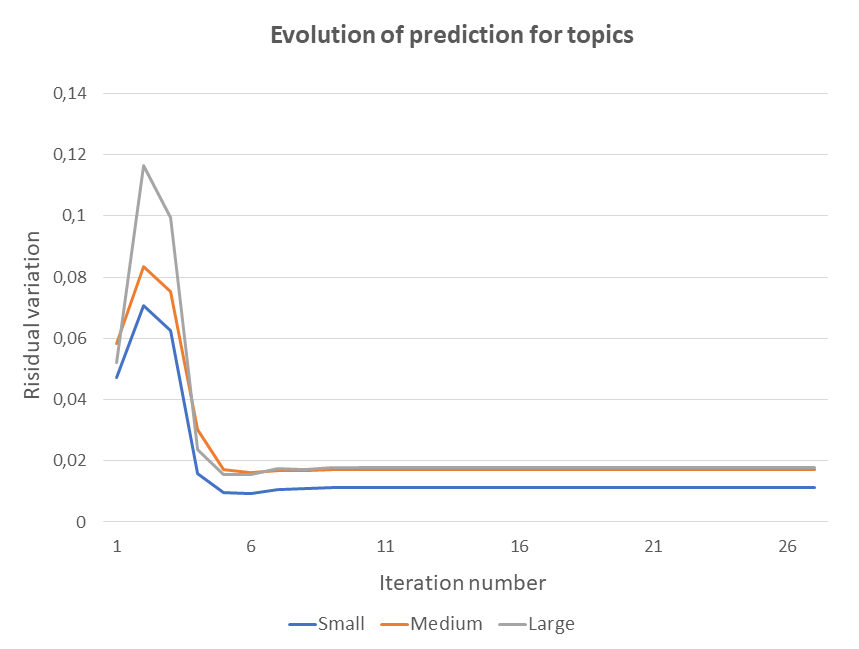
\includegraphics[width=\linewidth]{figs/total}}
		\caption{Resudial variation computed between the real value of power and the guessed one at each dialogue turn} 
		\label{fig:converge}
	\end{figure}
	
	
	\subsubsection{Timeliness}
	We evaluate the time execution of the algorithm in order to study how the model of theory of mind evolves. For each dialogue, we computed the average time execution at each negotiation turn. We aim to study the effect of hypotheses's size on the rapidity of prediction at each turn. Results are presented in figure \ref{fig:time}. When comparing the time execution between the medium and large models, we observe that the algorithm took in average $12$ milliseconds at each turn. However, this difference is not significant since the total execution remains very quick.
	
	\begin{figure}[]
		\fbox{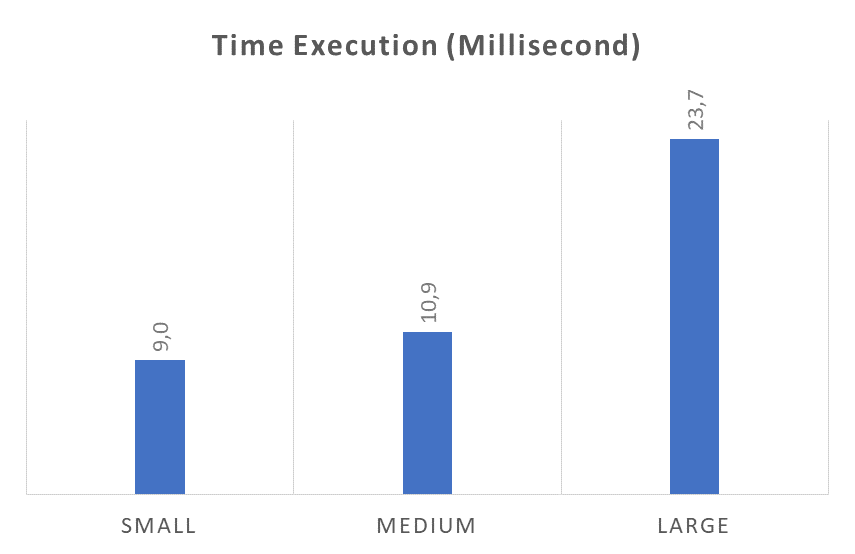
\includegraphics[width=\linewidth]{figs/time_exec.png}}
		\caption{Iime execution of the ToM algorithm at each dialogue turn} 
		\label{fig:time}
	\end{figure}
	
	We analyzed the behaviors of our model of ToM in different aspects and the obtained results provide a strong support to its accuracy. Indeed, for most of the generated dialogue, the agent with ToM abilities was able to predict a very close approximation of its partner's level of power. Moreover, the agent was able to find the right dominance range only after two speaking turns and the best evaluation after five turns. These behaviors were generated in a reasonable amount of time, allowing the agent to produce real time dialogues.
	
	These findings strengthen the accuracy of our model and give good perspectives to implement this model in the context of human/ agent collaborative negotiation. However, the presented validation in the context of agent/agent negotiation is a controlled evaluation since both agents use the same decisional model. This situation increases the chance of good predictions of the partner's behaviors of power. 	
	Thus, our collaborative model of negotiation must be validated in the context of human/agent negotiation. Our initial model of power \cite{ouali2017computational} relies on studies from social psychology. It has been validated with a perceptive study where human participants were able to perceive and recognize behaviors of power expressed by agents. For these reasons, we believe that it is a good approximation of human behaviors of power and we expect good predictions from our ToM model in the context of human-agent interaction.

	\section{Conclusion}
			
	We presented in this paper, a model of collaborative negotiation enabled with a simulation model in order to predict the behavior of the interlocutor. Our aim, is to enable a conversational agent to guess the behavior of its interlocutor in order to adopt a complementary behavior.
	
	 Our model of ToM focuses essentially on predicting the behavior of power expressed by the agent's interlocutor. To this purpose, we used simulation theory (\emph{ST}). It assumes that the agent is capable to reason from the perspective of its interlocutor using his own mechanism of reasoning and decision.
	  
	We presented a solution in which the agent builds a partial representation of the mental state of its interlocutor. This allows the agent to have sufficient knowledge to compute the value of the interlocutor's power. Our results are compatible with the research in cognitive psychology: \cite{harbers2009modeling} suggests that, in order to simulate another's mental processes, it is not necessary to categorize all the beliefs and desires attributed to that person as such. In other words, it is not necessary to have a complete model of the interlocutor.
	
	We adapted the decision process of the agent to handle partial knowledge and we presented an evaluation to validate the accuracy of the agent's prediction in the context of agent/agent negotiation. The results confirmed the accuracy of the ToM models. Indeed, the agent was able to generate, in a limited number of dialogue turns, an accurate prediction of it's partner behaviors.
	
	%Rappeler l'importance de la complementarite
	As perspective, we aim to simulate a complementary relation of dominance between an agent and human user during a process of collaborative negotiation. In such case, the agent will have to adapt its behaviors of power to complement the predicted user's behaviors in order to simulate the dominance complementarity. Thus, the agent will have to consider the effect of wrong predictions on the negotiation outcomes. We believe that modeling a complementary relation of dominance will improve the negotiation outcomes and increase mutual liking between the agent and the user similarly to human/human negotiations \cite{wiltermuth2015benefits,tiedens2003power}.
	
	\bibliographystyle{IEEEtran}
	% argument is your BibTeX string definitions and bibliography database(s)
	\bibliography{bibliography}
	%
	% <OR> manually copy in the resultant .bbl file
	% set second argument of \begin to the number of references
	% (used to reserve space for the reference number labels box)
	
	
	
	
	
	% that's all folks
	\end{document}
	
	
